\documentclass[12pt,a4paper,titlepage]{article}

\usepackage[top=0.8in, bottom=0.8in, left=0.2in, right=0.2in]{geometry}
\usepackage{subfigure}
\usepackage{graphicx}
\usepackage{float}
\usepackage[hidelinks]{hyperref}
\usepackage[AutoFakeBold=true]{xeCJK}
\usepackage{algorithm}
\usepackage{algorithmicx}
\usepackage{algpseudocode}
\usepackage{listings}
\usepackage{color}
\usepackage{tikz}
\usepackage{indentfirst}
\usepackage{enumitem} 
\usepackage[hyperref]{ntheorem}
\usepackage{fancyhdr}
\usepackage{amsmath,amssymb}
\usepackage[toc,page]{appendix}
\usepackage{multirow}
\usepackage{cite}
\usepackage{changepage}

%\setmainfont{DejaVu Sans}
\setCJKsansfont{等线}
\setCJKmainfont{SimSun}
\setmainfont{Times New Roman}
\newfloat{figtab}{htb}{fgtb}
\makeatletter
    \newcommand\figcaption{\def\@captype{figure}\caption}
    \newcommand\tabcaption{\def\@captype{table}\caption}
\makeatother

\bibliographystyle{ieeetr}

\definecolor{mygreen}{rgb}{0,0.6,0}
\definecolor{mygray}{rgb}{0.5,0.5,0.5}
\definecolor{mymauve}{rgb}{0.58,0,0.82}

\setlength{\parindent}{2em}

\lstset{
	language=C++,
	numbers=left,
	breaklines=true,
	basicstyle=\scriptsize,
	commentstyle=\color{mygreen},
	keywordstyle=\color{blue},
	numberstyle=\color{mygray},
	rulecolor=\color{black},
	stringstyle=\color{mymauve}
}

\pagestyle{fancy}
\lhead{\leftmark}
\rhead{不经意随机访问机综述}
\renewcommand{\headrulewidth}{0.5pt}


\theoremstyle{plain}
\theoremsymbol{\ensuremath{\clubsuit}}
\theoremseparator{.}
\theoremprework{\bigskip\hrule}
\theorempostwork{\hrule\bigskip}
\theoremindent1em
\newtheorem{definition}{定义}[section]

%\newtheorem{definition}{\hspace{2em}\textbf{定义}}[section]
\newtheorem{theorem}{定理}[section]

\title{
	
\includegraphics[scale=1.5]{zju_1.pdf}\\~\\
	
\includegraphics[scale=1]{zju_2.pdf}\\
	~\\
	\Huge{不经意随机访问机综述}\\[2ex]
	\sffamily\large{面向信息技术的沟通技巧---作业3}
}
\author{
	Zhu Jingsen\\
	朱璟森\\
	3170104166
}

\newcommand{\enabstractname}{Abstract}
\newenvironment{enabstract}{%
    \par
    \noindent\mbox{}\hfill{\bfseries \enabstractname}\hfill\mbox{}\par\vskip 1ex\begin{adjustwidth}{2em}{2em}
	}{\par\vskip 2.5ex\end{adjustwidth}}  

\setlength{\parskip}{0.1em}
\linespread{1.1}
\setenumerate[1]{itemsep=0pt,partopsep=0pt,parsep=5pt,topsep=5pt}
\setitemize[1]{itemsep=0pt,partopsep=0pt,parsep=5pt,topsep=5pt}
\setdescription{itemsep=0pt,partopsep=0pt,parsep=5pt,topsep=5pt}
	
\begin{document}
	\maketitle
	\newpage
	\tableofcontents
	\newpage

	\begin{enabstract}
		\raggedright
		With the development of cloud computing, more and more people and companies choose to store their data in cloud servers, which cause potential safety hazards. Despite the use of strong encryption schemes, adversaries can still learn valuable information regarding encrypted data by observing the data access patterns. In solution, one can hide the access patterns, which may leak sensitive information, using Oblivious RAMs (ORAMs). There are many implementations of ORAMs to hide the access patterns. A main issue remains to decrease the time and bandwidth costs. In this review, we list several implementations of ORAMs and summerize their performences.
		\par
		\textbf{Keywords:} Access pattern, ORAM, cloud computing
	\end{enabstract}
	\section{背景与定义}
\subsection{背景---访问模式与数据安全\cite{ref0,ref00}}\par
随着云计算、云服务的发展,越来越多的数据被存储在云端服务器上。然而,一旦服务器遭到恶意攻击,或者不可信的云服务提供商恶意获取服务器信息,用户的隐私信息就会泄露。传统的手段是对数据内容进行加密,密钥由用户个人持有.用户通过上传、下载密文数据来保护个人的隐私信息不被泄露。\par
然而,加密只能保证数据内容的机密性,由于CPU与内存之间的内存总线 (Address Bus) 是无法加密的,攻击者通过客户端访问的数据块地址序列(访问模式),依旧能够推断出其它的隐私信息。如文献\cite{ref1}中,攻击者可以通过搜集访问模式,可以通过统计的手段推断出80\%已加密的搜索请求。而在逆向工程领域\cite{ref2,ref3},内存地址的访问模式可以帮助攻击者分析出程序的结构,例如,在程序运行的过程中,攻击者可以观察到对内存位置100,101,X(102或103),104重复出现,他就可以推断出这是一个包含着条件分支的循环。
\begin{figure}[H]
    \centering
    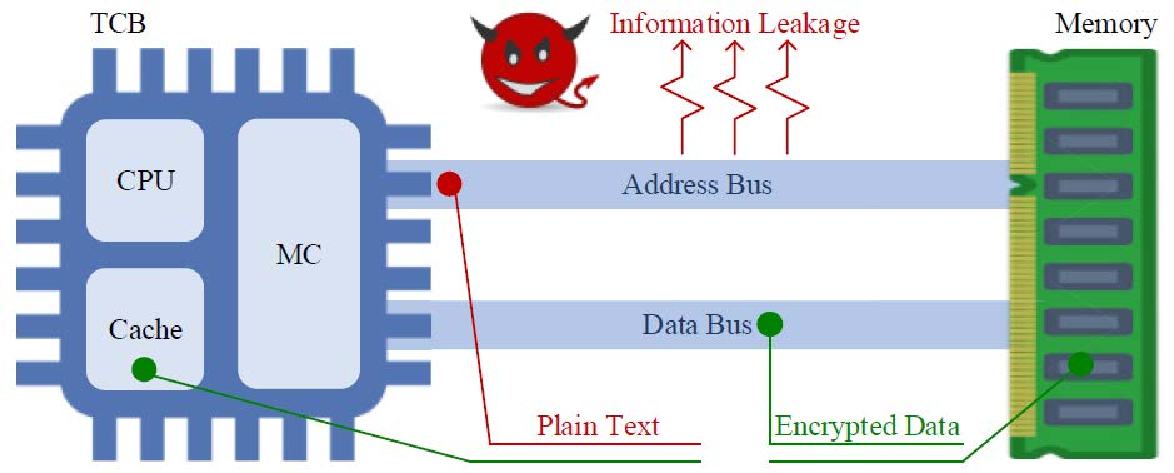
\includegraphics[width=0.8\textwidth]{introduction/leakage.pdf}
    \caption{内存总线上访问模式的泄露}
    \label{fig:leak}
\end{figure}
Goldreich与Ostrovsky在论文中\cite{ref4}提出了不经意随机访问机 (Oblivious RAM, abbr. ORAM)技术。这一技术的目的是隐藏对真实数据块的访问,使得攻击者不能区分每一次访问是真实的还是随机的。不经意随机访问机应用于云存储系统可以有效的防止攻击者利用访问模式获取隐私信息,减小数据存储系统的攻击面,打破了单纯使用传统加密方式来保护数据隐私的系统框架,为用户提供更完善的安全存储服务。\par%
但是,不经意随机访问机也会带来额外的开销,比如:为了隐藏访问模式,需要对多个数据块进行访问,这增大了客户端与服务器之间的带宽,客户端需要更大的缓存空间来存储从服务器端返回的额外数据块。所以,不经意随机访问机的实用性还面临很大的挑战。
\subsection{ORAM安全性定义}\par
为保护和混淆内存的访问模式,ORAM 保证了在存储器中的任意数据块不会永久驻留在某一个物理地址中,这确保了任意两次访问不会产生关联。同时,ORAM将每一次读写访问 (access) 细化成一次读取加一次写回的原子操作 (operation) ,其中读问转化成读取内容再写回相同内容,写访问转化成读取内容再写回更新后的内容,使得攻击者不能够区分具体的访问方式。ORAM能很好地保护
\begin{enumerate}
    \item 访问数据块的位置
    \item 数据块请求的顺序
    \item 对相同数据块的访问频率
    \item 具体的读写访问方式
\end{enumerate}
\par\noindent 下面我们对ORAM的安全性进行正式的定义:
\begin{definition}\textbf{ORAM安全性}
    \newline
    设$\vec{y}$为长度为$M$的一系列数据操作序列,$\vec{y}=(op_1,id_1,block_1),\ldots,(op_M,id_M,block_M)$,$op_i$为读操作$read(id_i)$,其读取标识符为$id_i$的块;或写操作$write(id_i,block_i)$,将新数据$block_i$写入到标识符为$id_i$的块中。如果$op_i=read(id_i)$,那么$block_i=null$。
    \newline
    给定操作序列$\vec{y}$,设其经过ORAM加密后的访问模式为$A(\vec{y})$,该ORAM体制是安全的当期仅当对任意两个相同长度序列$\vec{y}, \vec{y'}$,其访问模式$A(\vec{y}), A(\vec{y'})$计算上不可区分。
\end{definition}\par
为了让读写操作不可区分,标准的解决方案是始终采用“先读后写”的操作,不需要写入的时候通过写入无效信息 (dummy write) 来进行混淆。
\subsection{发展脉络}
不经意随机访问机的概念最早起源于RAM (random access machine)模型,RAM是一种重要的计算仿真手段。在这个模型中,处理器通过对存储器的读写来实现程序的执行。上个世纪80年代,为了隐藏程序对内存的访问模式来避免软件的逆向工程,Goldriche等人在此基础上提出了ORAM\cite{ref2},开启了ORAM的研究历程。不经意随机访问机面临的最大问题是性能开销大。纵观不经意随机访问机的发展。其设计模型大致可以分为5类:简单模型、平方根模型\cite{ref5,ref6}、层次模型\cite{ref5}、分区模型\cite{ref7}和树状模型\cite{ref8,ref9}。不同的设计模型表示服务器存储数据块的数据结构不同,用户通过对服务器ORAM的访问来获取所需的数据块,这些模型设计的目标主要还是提高性能。本文主要介绍后4种模型及其变种,并简介ORAM的最新研究进展。
	\section{常见ORAM体制研究进展}
\subsection{ORAM常用的技术}
\subsubsection{不经意排序}
\textit{不经意排序 (Oblivious sort)},又称为茫然排序,是指这样一种排序算法,其排序过程对数据操作的顺序是\textit{预定义、固定的},如冒泡排序是典型的茫然排序,而选择排序则不是 (顺序依赖于数据中每一轮的最大值) 。时间复杂性较好的茫然排序有$O(n\log^2{n})$的Batcher排序网络和$O(n\log{n})$的AKS排序网络,然而后者的常数项 ($\approx{6100}$) 远大于前者 ($\approx{0.5}$) ,因此实用中通常采用理论复杂度更高的前者。
\subsubsection{不经意随机排列}
\textit{不经意随机排列 (Oblivious random permutation)},在许多ORAM体制对数据的预处理与混洗 (shuffle) 中用到。我们通常采用Knuth洗牌算法:
\begin{algorithm}[H]
    \label{alg:Knuth}
    \caption{Knuth shuffle algorithm}
    \begin{algorithmic}[1]
        \Procedure {shuffle}{$A,N$}
            \For{$i \gets 0 \ \mathbf{to}\ N-1$}
                \State $j \gets random(0,N-1)$
                \State \Call{swap}{$A_i,A_j$}
            \EndFor
		\EndProcedure
    \end{algorithmic}
\end{algorithm}

\subsection{平方根模型}
\textit{Square Root ORAM}是第一个在文献中提出的ORAM模型\cite{ref5},分为\textit{Basic Square Root ORAM (Basic-SR)}及其改进\textit{Interleave Buffer Shuffle Square Root ORAM (IBS-SR)}。
\subsubsection{Basic-SR}
在这个ORAM中,服务器的结构如下:服务器共储存$N+2\sqrt{N}$个数据块,其中$N$个为加密过的真实数据块,$\sqrt{N}$个为用于混淆的伪数据块(dummy block),最后$N$个为缓冲区(shelter)。\par
\noindent Basic-SR的算法流程如下:
\begin{enumerate}
    \item 对前$N+\sqrt N$个数据块,也就是真实数据块与伪数据块一起进行随机排列。
    \item 扫描缓冲区$\sqrt N$个数据块
    \begin{itemize}
        \item $j$在缓冲区中,则对缓冲区进行一次伪数据块读写
        \item $j$不在缓冲区中,则从$j$的位置$\pi(id_j)$中读取数据并写入伪数据块
    \end{itemize}
    \item 进行第二次缓冲区扫描,如果是写操作就在缓冲区中更新数据,读操作就写入伪数据块。
    \item 当计数器$count$增加到$\sqrt N$时,就要对所有数据块进行不经意排序,否则访问模式就会有泄漏的风险。
\end{enumerate}
伪代码如下:
\begin{algorithm}[H]
    \label{alg:BSR}
    \caption{Basic-SR ORAM}
    \begin{algorithmic}[1]
        \State $p \gets 0$
        \While{\textbf{true}}
            \State $p \gets p+1$
            \State Perform an oblivious random permutation $\pi$ of the blocks in the first $(N + \sqrt N)$ locations (data + dummy blocks)
            \For{$count \gets 1\ \mathbf{to}\ \sqrt N$}
                \State $j\gets (p-1)\sqrt N+count$
                \If{$id_j$ in shelter location $x\ (N+\sqrt N+1\leq x\leq N+2\sqrt N)$}
                    \State Read a dummy block from $\pi(N+count)$
                    \State Write back this dummy block
                \Else\Comment{$id_j$ not in shelter}
                    \State $x\gets -1$, read $id_j$ from $\pi(id_j)$
                    \State Write a dummy block to $\pi(id_j)$
                \EndIf
                \For{$i\ \gets 1\ \mathbf{to}\ \sqrt N$}\Comment{scan the shelter}
                    \State Read shelter block $N+\sqrt N+i$
                    \If{$N+\sqrt N+i=x$}
                        \If{$op_j=write$}
                            \State Write $block_j$ to $N+\sqrt N+i$
                        \Else\Comment{$op_j=read$}
                            \State Write the same data back to $N+\sqrt N+i$
                        \EndIf
                    \ElsIf{$i=count \and x=-1$}
                        \If{$op_j=write$}
                            \State Write $block_j$ to $N+\sqrt N+i$
                        \Else\Comment{$op_j=read$}
                            \State Write the same data back to $N+\sqrt N+i$
                        \EndIf
                    \Else
                        \State Write a dummy block to $N+\sqrt N+i=x$
                    \EndIf
                \EndFor
            \EndFor
            \State Perform an oblivious sort on all $(N + 2\sqrt N)$ locations
        \EndWhile
    \end{algorithmic}
\end{algorithm}
平方根模型以$\sqrt N$次访问为一轮。在每一轮访问中,保证前面每个数据块的位置只会被访问一次,之后被访问的数据块就会被载入缓冲区shelter中。而对缓冲区shelter的查找与访问都会扫描整个缓冲区,以保证不会泄露访问模式。每一轮访问结束之后,所有数据就要重新排序混洗。\par
Basic-SR ORAM模型,对每一轮访问($\sqrt N$次),摊还时间复杂度由不经意排序的复杂度决定,为$O(\sqrt N\log^2 N)$(Batcher排序网络)或$O(\sqrt N\log N)$(AKS排序网络)。
\subsubsection{IBS-SR}
IBS-SR是对平方根模型的一个简要改进\cite{ref6},服务器储存$N$个数据块和$\sqrt N$个伪数据块,而对客户端有$O(\sqrt N)$的内存空间复杂度。\par
IBS-SR的改进在于,使用哈希函数,每次对哈希映射到的$\sqrt{N+\sqrt{N}}$个数据块进行混洗并更换哈希映射,以代替Basic-SR中$O(N\log^2 N)$的不经意排序操作,该混洗操作称为\textit{Interleave Buffer Shuffle (IBS)}。从而突破了不经意排序的性能瓶颈,使得ORAM的摊还时间复杂度降为$O(\sqrt{N})$。

\subsection{层次模型}
\textit{Hierarchical ORAM}是文献\cite{ref5}中提出的另一种ORAM,相比Square Root ORAM,Hierarchical ORAM的效率比较高。\par
\textit{Basic Hierarchical ORAM (Basic-HR)}将服务器存储空间划分为$L=\lceil\log_2N\rceil$层,每层$\ell (1\leq\ell\leq L)$中有$2^\ell$个桶,则每层的桶的个数恰好是上一层中的两倍。每$2^\ell$次操作后,第$\ell$层就会被混洗。初始化的时候,要为每一层选择一个hash函数,用于决定数据块应放入哪个桶中。
\begin{figure}[H]
    \centering
    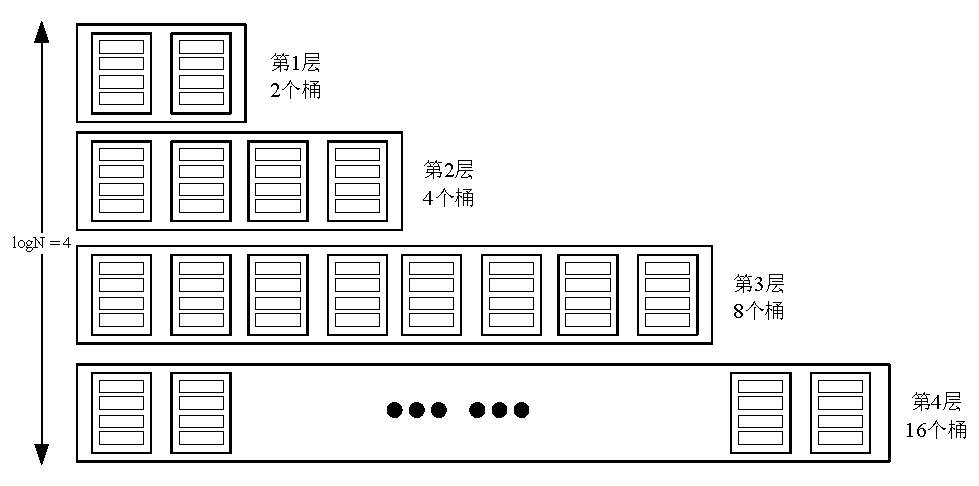
\includegraphics[width=0.8\textwidth]{orams/hierarchical.pdf}
    \caption{$L=4$时Hierarchical ORAM的数据结构}
    \label{fig:hier}
\end{figure}
Basic-HR算法流程如下:
\begin{enumerate}
    \item 从第1层到第L层,逐层根据哈希函数扫描数据块$id_j$可能在的桶。如果在之前的层中已经找到,则随机选一个桶来读写。如果在该层找到,则读取后写回一个伪数据块。如果没有找到,则读取并原样写回该桶的数据块。
    \item 所有层搜索完毕后,将数据块$id_j$写入第一层。
    \item 每进行$2^\ell$次操作,就要将$\ell$层与$\ell+1$层数据块混洗,并且哈希函数要重新选取。
\end{enumerate}
伪代码如下:
\begin{algorithm}[H]
    \label{alg:BHR}
    \caption{Basic-HR ORAM}
    \begin{algorithmic}[1]
        \State $j \gets 0$
        \While{\textbf{true}}
            \State $j \gets j+1$
            \For{$\ell \gets 1\ \mathbf{to}\ L$}
                \If{block $id_j$ hasn't been found}
                    \State Scan hash bucket to find $id_j$
                    \If{$id_j$ found}
                        \State Write a dummy block back
                    \Else
                        \State Write the original block back
                    \EndIf
                \Else\Comment{$id_j$ has been found}
                    \State Read and write a random block in level $\ell$
                \EndIf
            \EndFor
            \If{$j$ is odd}
                \State Write block $id_j$ into 1st bucket in level 1.
            \Else
                \State Write block $id_j$ into 2nd bucket in level 1.
            \EndIf
            \State $d \gets \max\{1\leq x\leq L: j\bmod 2^x = 0\}$
            \For{$\ell \gets 1\ \mathbf{to}\ d$}\Comment{shuffle every $2^\ell$ operations}
                \State Pick a new hash function for level $\ell+1$
                \State Shuffle data in level $\ell$ and level $\ell+1$ using the new hash function.
            \EndFor
        \EndWhile
    \end{algorithmic}
\end{algorithm}
复杂度分析上,云端服务器的空间开销为$O(N\log N)$,客户端空间开销为$O(1)$。摊还时间复杂度由不经意排序的复杂度决定,为$O(\log^4 N)$(Batcher排序网络)或$O(\log^3 N)$(AKS排序网络)。与平方根模型相比有显著提升,但仍开销较大。

\subsection{分区模型}
\textit{TP-ORAM}是文献\cite{ref7}中提出的一种对层次模型的改进,其核心思想为将服务器分区(partition),将单个大小$N$分割为$\sqrt N$个小型ORAM,每个分区相当于一个ORAM的黑盒子,并不依赖具体的内部实现。\par
TP-ORAM中,分为$P=\sqrt{N}$个分区,每个分区采用层次模型,因此每个分区内有$L=\log_2{\sqrt{N}}+1=\frac{1}{2}\log_2N+1$层。与Basic-HR一样,第$\ell$层有$2^\ell$个块。为了防止随机误差导致的可能溢出,第$L$层有$2^L+\epsilon=2\sqrt{N}+\epsilon$个区块。通过简单的几何级数求和可以知道,每个分区一共有$4\sqrt{N}-2+\epsilon$个区块,而在具体实现\cite{ref7}中,被进一步放宽为$4.6\sqrt{N}$。除了分块内存,服务器中还存在$O(\sqrt{N})$大小的缓冲区(stash),stash被分为$P$块,每块对应服务器内存的一个分区。另外还有一个映射表(position map)来决定每一个数据块$id_j$被分配到哪个分区中。
\begin{figure}[H]
    \centering
    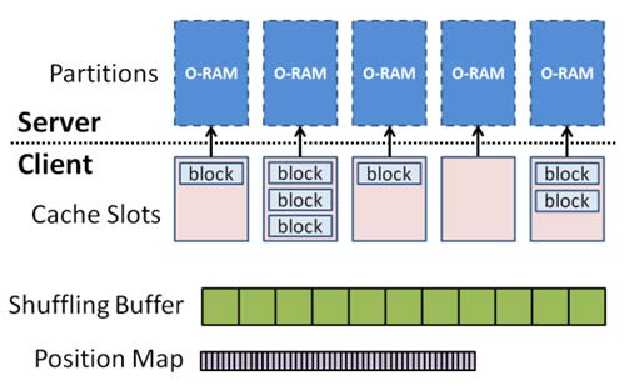
\includegraphics[width=0.8\textwidth]{orams/partition.pdf}
    \caption{分区模型的数据结构}
    \label{fig:part}
\end{figure}
\noindent TP-ORAM的主要流程如下:
\begin{enumerate}
    \item 通过映射表获取$id_j$所在的分区。先访问缓冲区,如果找到就读取出来并对内存分区进行一次伪访问;否则从内存分区中访问$id_j$。
    \item 随机选择另一个分区编号$r$,更新映射表并将$id_j$放到新的缓冲区中。
    \item 进行两次驱逐操作。
\end{enumerate}
伪代码如下:
\begin{algorithm}[H]
    \label{alg:TP}
    \caption{TP-ORAM}
    \begin{algorithmic}[1]
        \State $j \gets 0, s \gets 1$
        \While{\textbf{true}}
            \State $j \gets j+1$
            \State $p \gets position[id_j]$
            \If{block $id_j$ found in $stash[p]$}
                \State Read and delete $id_j$ from $stash[p]$
                \State Read a dummy block from partition $p$
            \Else\Comment{$id_j$ not in stash}
                \State Read $id_j$ from partition $p$
            \EndIf
            \State $r \gets random(1,P)$
            \State $position[id_j] \gets r$
            \State add $id_j$ into $stash[r]$
            \State\Call{Evict}{p} \Comment{Piggy-backed eviction}
            \State\Call{SequentialEvict}{$\nu$} or \Call{RandomEvict}{$\nu$}
        \EndWhile
    \end{algorithmic}
\end{algorithm}
驱逐操作(eviction)分为两个过程,第一个eviction过程是捎带式(Piggy-backed)的,也就是客户端执行一次访问之后,就会执行一次驱逐操作。驱逐操作将缓冲区中的一个元素“驱逐”回内存分区中,并对缓冲区写入一个伪数据。\par
第二步称为背景式(Background)驱逐,取决于一个频率参数$\nu$,每次数据访问之后,都会执行$\nu$次eviction操作。如果$\nu<1$说明多次访问之后才会执行一次背景式eviction操作。而背景式eviction操作有两种策略,一种是顺序驱逐,另一种是随机驱逐。
\begin{algorithm}[H]
    \caption{Evict}
    \begin{algorithmic}[1]
        \Procedure{Evict}{$p$}
            \If{$stash[p]$ is empty}
                \State Write a dummy block to partition $p$
            \Else
                \State Write a block from $stash[p]$ to partition $p$ and remove it from $stash[p]$
            \EndIf
        \EndProcedure
    \end{algorithmic}
\end{algorithm}
\begin{algorithm}[H]
    \caption{Sequential and Random Evict}
    \begin{minipage}{0.5\textwidth}
        \begin{algorithmic}[1]
            \Procedure{SequentialEvict}{$\nu$}
                \State $num \gets \mathcal{D}(\nu)$
                \Comment{$\mathcal{D}$ is a prescribed distribution}
                \For{$i \gets 1\ \mathbf{to}\ num$}
                    \State $count \gets count+1$
                    \State\Call{Evict}{$count$}
                \EndFor
            \EndProcedure
        \end{algorithmic}
    \end{minipage}
    \begin{minipage}{0.5\textwidth}
        \begin{algorithmic}[1]
            \Procedure{RandomEvict}{$\nu$}
                \State $num \gets \mathcal{D}(\nu)$
                \For{$i \gets 1\ \mathbf{to}\ num$}
                    \State $r \gets random(1,P)$
                    \State\Call{Evict}{$r$}
                \EndFor
            \EndProcedure
        \end{algorithmic}
    \end{minipage}
\end{algorithm}
复杂度分析上,云端服务器的空间开销为$O(N)$,客户端空间开销为$O(\sqrt{N}+\frac{N}{B})$,$O(\sqrt{N})$为缓冲区而$O(\frac{N}{B})$为映射表($B$为每个数据块的大小)。摊还时间复杂度可以低至$O(\log N)$,最坏情况为$O(\sqrt{N})$。分区模型相比于传统的模型而言有着显著的提升,但最坏情况依然开销较大。

\subsection{Basic Binary-Tree ORAM}
文献\cite{ref8}中提出了一种全新的树状模型,它不需要进行不经意排序和混洗操作,可以将ORAM操作的\textbf{最坏时间复杂度}控制在对数多项式以内,完成了一次显著的突破。\par
\textit{Basic Binary-Tree ORAM (BB-ORAM)}将整个服务器存储看做一棵平衡二叉树,而每个数据块映射到二叉树的每个叶节点。同时,客户端需要维护一个映射表(position map)来确定每个数据块所在的节点。

\subsection{Path-ORAM}
\textit{Path-ORAM}是文献\cite{ref9}中对BB-ORAM的一种改进,其思想同样采用树状模型,而在实现细节上有所优化。\par
与BB-ORAM一样,Path-ORAM把整个服务器存储看做一棵高为$L=\lfloor\log N\rfloor$的二叉树,树上的每个节点上有一个大小为$Z$的桶(bucket),其中含有真实数据块与伪数据块。每一个叶子节点$x\in\{0,1,\ldots,2^L-1\}$可以唯一确定一条从根到叶子的路径,令$\mathcal{P}(x)$为路径上所有桶的集合,特别地,$\mathcal{P}(x,\ell)$表示路径上第$\ell$层的桶。另外,客户端上有一块$O(\log N)$的缓冲区(stash),以及需要维护一块$O(\frac{N}{B})$的映射表。
\begin{figure}
    \centering
    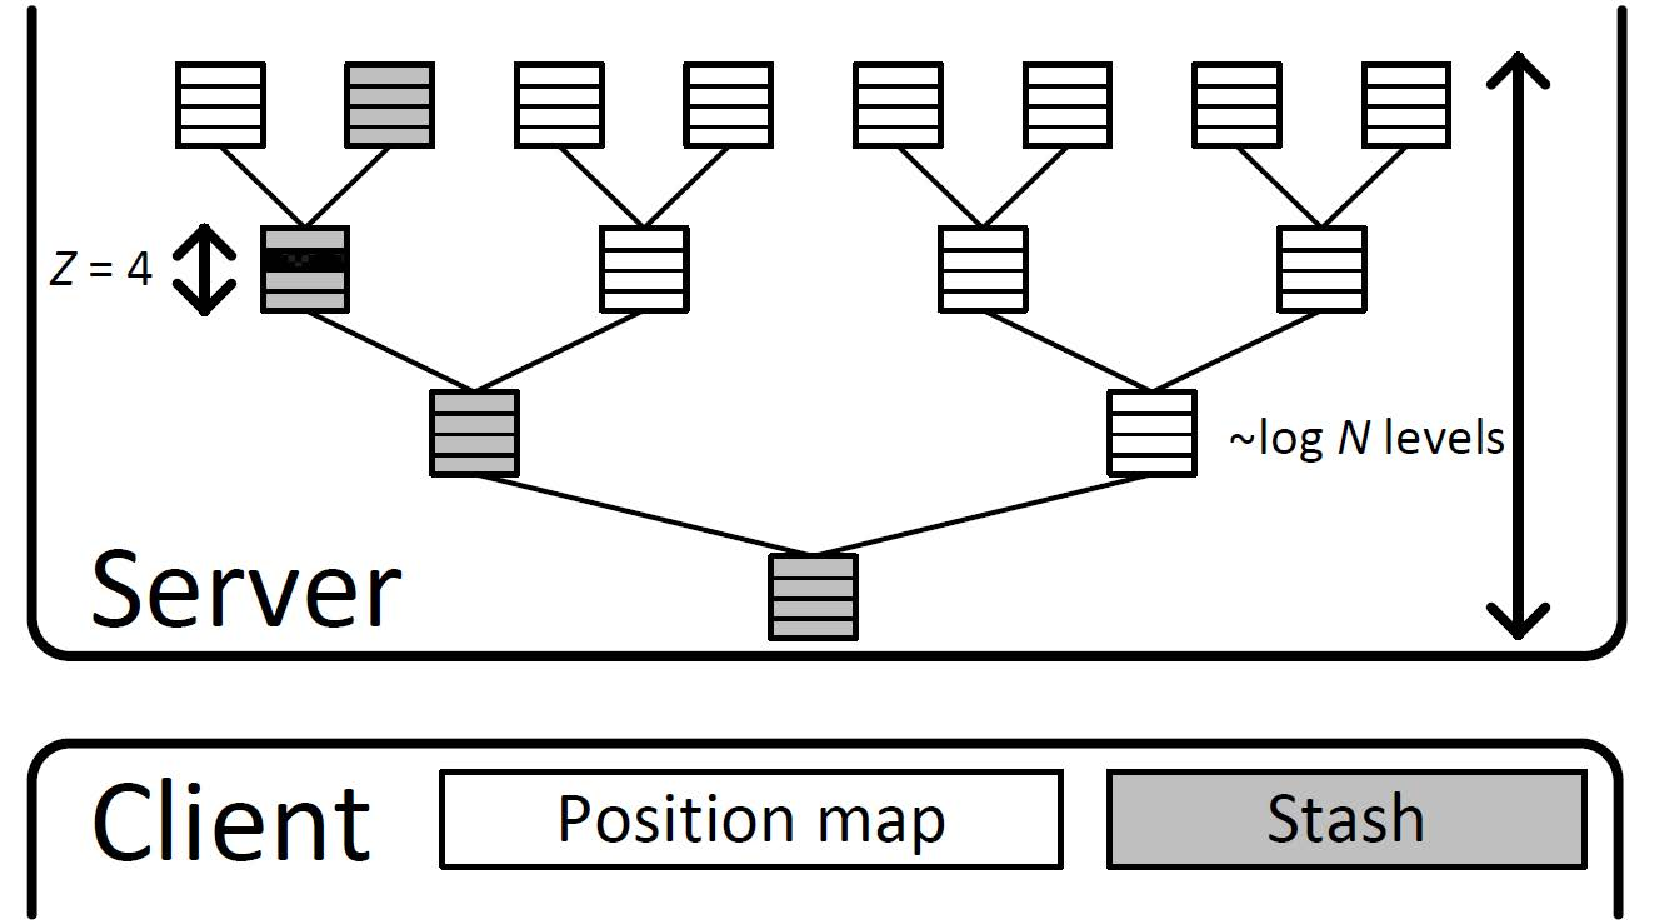
\includegraphics[width=0.65\textwidth]{orams/path.pdf}
    \caption{Path-ORAM的树状结构}
    \label{fig:path}
\end{figure}
\noindent Path-ORAM的算法流程如下:
\begin{enumerate}
    \item 通过映射表获取$id_j$所对应的叶节点$x$,并更新映射表,将$id_j$随机重新映射到另一个叶节点上。
    \item 将路径$\mathcal{P}(x)$上的所有桶全部读取到缓冲区中
    \item 如果是写操作,则写入$block_j$
    \item 将缓冲区中的数据尽可能写入回$\mathcal{P}(x)$中,其中一些本来不映射到$x$的数据也可能写入到第$\ell$层,只要$\mathcal{P}(x,\ell)=\mathcal{P}(x',\ell)$,即$x$路径与$x'$路径在第$\ell$层之前部分重合,那么该数据也可以写入到$\mathcal{P}(x,\ell)$中。
\end{enumerate}\par
这样,在服务端看来,客户端每次访问都是读取并写入一条随机的路径,因此访问模式不会被泄露。伪代码如下:
\begin{algorithm}[H]
    \label{alg:Path}
    \caption{Path-ORAM}
    \begin{algorithmic}[1]
        \State $j \gets 0, s \gets 1$
        \While{\textbf{true}}
            \State $j \gets j+1$
            \State $x \gets position[id_j]$
            \State $position[id_j] \gets random(0,2^L-1)$
            \For{$\ell \gets 0\ \mathbf{to}\ L$}
                \State $S \gets S \cup \mathcal{P}(x,\ell)$\Comment{$S$ denotes the stash}
            \EndFor
            \State data $\gets$ Read $id_j$ from $S$
            \If{$op_j=write$}
                \State $S \gets (S-\{(id_j,data)\})\cup\{(id_j,block_j)\}$\Comment{update old data to $block_j$}
            \EndIf
            \For{$\ell \gets L\ \mathbf{to}\ 0$}
                \State $S' \gets \{(a',data')\in S: \mathcal{P}(x,\ell)=\mathcal{P}(position[a'],\ell)\}$
                \Comment{$S'$ denotes the datas to write back in level $\ell$}
                \State $S' \gets$ Select $\min(|S'|,Z)$ from $S'$
                \State $S \gets S - S'$
                \State Write $S'$ into bucket $\mathcal{P}(x,\ell)$
            \EndFor
        \EndWhile
    \end{algorithmic}
\end{algorithm}
Path-ORAM原理简单,却极其高效,而二叉树的良好特性使其复杂度比之前的模型有了明显的提升。服务端空间需求为$O(N)$,而客户端的空间需求为$O(\log N+\frac{N}{B})$,即缓冲区加上映射表的大小。\par
时间复杂度方面,由于每次操作只需遍历一条路径,则平均与最坏时间复杂度都与树的高度成正比,即$O(\log N)$。带宽的消耗也优化到了对数级别,总带宽为$O(\frac{\log^2N}{\log B})$,平均带宽为$O(\frac{\log N}{\log B})$,只要$B=\Omega(\log^2N)$,Path-ORAM将比之前所有的ORAM模型拥有更低的复杂度\cite{ref9}。
	\section{总结与展望}
\subsection{ORAM小结}
\subsubsection{优劣分析}
表\ref{tab:adv}中,列出了几种ORAM模型的优缺点。
\begin{table}[H]
    \centering
    \begin{tabular}{|c|p{0.4\textwidth}|p{0.4\textwidth}|}
        \hline
        ORAM Type&优点&缺点\\
        \hline
        \multirow{3}*{Basic-SR}&\multirow{3}*{只需要访问缓冲区中的数据,带宽较低}&(1)需要复杂的混洗(不经意排序)操作,利用排序网络开销较大\\
        &&(2)平均带宽依然很高,不适用于具体应用\\
        \hline
        \multirow{2}*{IBS-SR}&\multirow{2}*{不需要不经意排序操作,开销降低}&(1)相比Basic-SR增加了客户端空间开销\\
        &&(2)复杂度$O(\sqrt{N})$不够理想\\
        \hline
        \multirow{4}*{层次模型}&\multirow{2}={(1)在平方根模型的基础上优化了带宽}&(1)依然需要复杂的混洗操作\\
        &\multirow{3}={(2)相比于平方根模型,层次模型考虑了每一个数据块被访问的频率}&(2)依据hash函数计算每一个数据块对应的数据块集合,容易导致hash值冲突;\\
        &&(3)平均带宽依然很高,不适用于具体应用\\
        \hline
        \multirow{3}*{分区模型}&\multirow{2}*{(1)分布式ORAM可以适用于云存储场景}&(1)需要更大的客户端存储空间\\
        &\multirow{2}*{(2)在层次模型上进一步优化了带宽}&(2)每一个服务器依然需要复杂的混洗操作,同时,驱逐操作也相对困难\\
        \hline
        \multirow{3}*{树状模型}&\multirow{3}={相比于平方根模型和层次模型,极大地降低了复杂度}&(1)驱逐操作的复杂度很高\\
        &&(2)客户端需要存储一个映射表,增大了客户端的存储空间\\
        \hline
    \end{tabular}
    \caption{几种ORAM模型的优缺点}
    \label{tab:adv}
\end{table}
\subsubsection{性能小结}
前文所述的是一些基本的ORAM架构,表\ref{tab:perf}对它们的性能进行了小结与比较,其中包括计算时间复杂度(摊还、最坏),通讯开销(摊还、最坏),以及服务器与客户端上消耗的空间存储。注:这里假设不经意排序采用$O(N\log^2N)$的Batcher排序网络。
\begin{table}[H]
    \centering
    \begin{tabular}{|c|c|c|c|c|c|c|}
        \hline
        \multirow{2}*{ORAM Type}& \multicolumn{2}{c|}{Computation Overhead}& \multirow{2}*{Cloud Storage}& \multicolumn{2}{c|}{Communication Overhead}& \multirow{2}*{Client Storage}\\
        \cline{2-3}\cline{5-6}
        &Amortized&Worst-Case&&Amortized&Worst-Case&\\
        \hline
        Basic-SR& $O(\sqrt{N}\log^2N)$& $O(N\log^2N)$& $O(N)$& $O(\sqrt{N}\log^2N)$& $O(N\log^2N)$& $O(1)$\\
        \hline
        IBS-SR& $O(\sqrt{N})$& $O(N)$& $O(N)$& $O(1)$& $O(\sqrt{N})$& $O(\sqrt{N})$\\
        \hline
        Basic-HR& $O(\log^4N)$& $O(N\log^3N)$& $O(N\log N)$& $O(\log^4N)$& $O(N\log^3N)$& $O(1)$\\
        \hline
        TP-ORAM& $O(\log N)$& $O(\sqrt N)$& $O(N)$& $O(1)$& $O(1)$& $O(\sqrt{N}+\frac{N}{B})$\\
        \hline
        BB-ORAM& $O(\log^2N)$& $O(\log^2N)$& $O(N\log N)$& $O(\log^2N)$& $O(\log^2N)$& $O(\frac{N}{B})$\\
        \hline
        Path-ORAM& $O(\log N)$& $O(\log N)$& $O(N)$& $O(\frac{\log^2 N}{\log B})$& $O(\frac{\log^2 N}{\log B})$& $O(\log N+\frac{N}{B})$\\
        \hline
    \end{tabular}
    \caption{几种ORAM模型的性能小结}
    \label{tab:perf}
\end{table}

\subsection{ORAM研究进展}
不同的ORAM模型各有优劣,其中,对当下的ORAM研究启发最大的是Hierarchical ORAM (Basic-HR)的层状结构、Path ORAM的树状结构与TP-ORAM的分区思想。ORAM的研究主要集中在减小ORAM的开销上,这是由ORAM本身的特点所决定的。ORAM主要应用于内存或存储系统,如果读写开销与存储开销太大,就会严重限制其实际应用。因此,前文所述ORAM研究主要是通过设计新的数据结构与算法,来降低ORAM的开销。\par
在这些研究的基础上,当下研究注重于结合各种ORAM模型的特点,改进已有的ORAM模型的算法与数据结构,运用新开发的技术,从细节上优化ORAM的带宽与存储开销、减少交互轮数、提高效率等。
\begin{enumerate}
    \item 如\cite{ref11}中提出的\textit{Ring ORAM}模型,对树状模型进行了进一步优化,其借鉴了Partition ORAM (TP-ORAM分区模型)的驱逐操作的思想,设置驱逐频率常数$A$,每$A$步后对路径和缓冲区进行一次驱逐操作,而不用像Path-ORAM那样每次都要讲Stash写回树中,首次使树状模型的复杂度独立于数据块大小$B$,比Path-ORAM效率提升了2.3到4倍\cite{ref11}。
    \item 而ObliviStore\cite{ref10}则是一个高性能、分布式的ORAM存储系统,提出分布式ORAM定义的同时,也实现了异步IO操作。
    \item 还有的模型\cite{ref12}使用有效数据的冗余来代替伪数据块,通过重复读写不同位置上的冗余数据来实现访问模式的混淆,将时间开销缩小到$O(1)$,然而其空间开销巨大(取决于冗余的程度)。
\end{enumerate}

\subsection{存在问题}
然而,虽然当下的ORAM研究已经取得了很大的进展,效率也有所提升,但依然有许多亟待解决的问题,这些问题限制了ORAM的实际应用,导致ORAM系统依然停留在理论研究上。
\begin{enumerate}
    \item ORAM的额外带宽开销依旧很大。如果要将ORAM部署于云环境上,则带宽开销会成为性能的主要瓶颈,严重影响ORAM的实用性。
    \item ORAM需要额外的客户端与服务端空间。ORAM系统在服务端不仅存储真实数据块,还会存储伪数据块,这造成了存储空间的浪费。而ORAM系统在客户端也常常需要存储缓冲区、映射表等,造成客户端空间的开销。
    \item ORAM的访问操作需要与服务端进行多轮交互。与带宽开销相似,这个缺点也会影响其在云环境下的应用性能,同时也会让ORAM的具体实现变得复杂。
    \item 当前支持分布式存储的ORAM极少,仅有少数(如上文提到的ObliviStore\cite{ref10})支持异步访问、并发访问的安全性,但其开销较大,限制了实际应用。
\end{enumerate}

\subsection{研究展望}
如前文所述,ORAM技术最主要的问题就是开销巨大,这导致其难以应用于实际。因此当前的研究着重提高其效率,降低其开销。除此之外,要实际应用ORAM技术还需要考虑更多问题,如分布式系统的同步、异步访问等等。具体来说,未来的ORAM研究可以注重以下几个方面。
\begin{enumerate}
    \item 在减小带宽开销方面还可以进行优化。云环境中,往往存储空间充足而传输带宽受到限制,如果带宽开销很大就会导致传输数据块的时间非常长,限制OARM的使用。当前,有的ORAM(如Onion-ORAM\cite{ref13})能使带宽开销降低到$O(1)$,但计算复杂度高。未来的研究可以尝试寻找其它的方式来达到$O(1)$的带宽开销。
    \item 在空间利用方面可以进行优化。当下的ORAM需要在服务端存储大量的伪数据块,这些伪数据块的内容没有意义,仅用于混淆真实数据块。但是,这样会造成空间的浪费。可以用利用伪数据块来存储一些信息,如\cite{ref12}的冗余思想,使伪数据块的内容有意义,提高空间的利用效率。
    \item 在分布式与并行访问方面进行研究。分布式与并行访问是云环境的一大特点,而真正实用的分布式ORAM系统还有待开发。
    \item 对ORAM模型的进一步完善。ORAM经典模型在上个世纪提出,这是一个简单的模型,只支持读写操作。未来可以针对实用性对ORAM模型进行进一步拓展,完善细节问题,如支持数据的删除与更新操作、满足分布式系统的一致性与可扩展性,实现日志功能等,从而推动ORAM系统的实际应用。
\end{enumerate}

	\bibliography{oram}

\end{document}
